\chapter{Algoritmos de árbol}

\index{árbol}

Un \key{árbol} es un grafo conectado y acíclico
que consiste en $n$ nodos y $n-1$ aristas.
Eliminar cualquier arista de un árbol lo divide
en dos componentes,
y agregar cualquier arista a un árbol crea un ciclo.
Además, siempre hay un camino único entre dos
nodos de un árbol.

Por ejemplo, el siguiente árbol consta de 8 nodos y 7 aristas:
\begin{center}
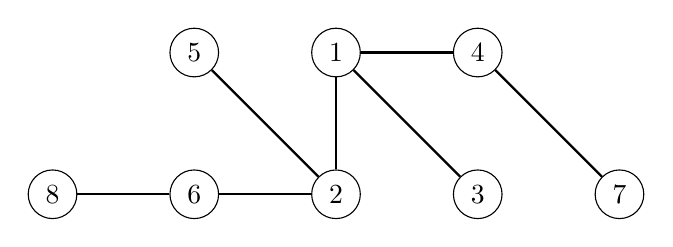
\begin{tikzpicture}[scale=0.9]
\node[draw, circle] (1) at (0,3) {$1$};
\node[draw, circle] (2) at (2,3) {$4$};
\node[draw, circle] (3) at (0,1) {$2$};
\node[draw, circle] (4) at (2,1) {$3$};
\node[draw, circle] (5) at (4,1) {$7$};
\node[draw, circle] (6) at (-2,3) {$5$};
\node[draw, circle] (7) at (-2,1) {$6$};
\node[draw, circle] (8) at (-4,1) {$8$};
\path[draw,thick,-] (1) -- (2);
\path[draw,thick,-] (1) -- (3);
\path[draw,thick,-] (1) -- (4);
\path[draw,thick,-] (2) -- (5);
\path[draw,thick,-] (3) -- (6);
\path[draw,thick,-] (3) -- (7);
\path[draw,thick,-] (7) -- (8);
\end{tikzpicture}
\end{center}

\index{hoja}

Las \key{hojas} de un árbol son los nodos
con grado 1, es decir, con solo un vecino.
Por ejemplo, las hojas del árbol anterior
son los nodos 3, 5, 7 y 8.

\index{raíz}
\index{árbol enraizado}

En un árbol \key{enraizado}, uno de los nodos
se designa como la \key{raíz} del árbol,
y todos los demás nodos se
colocan debajo de la raíz.
Por ejemplo, en el siguiente árbol,
el nodo 1 es el nodo raíz.

\begin{center}
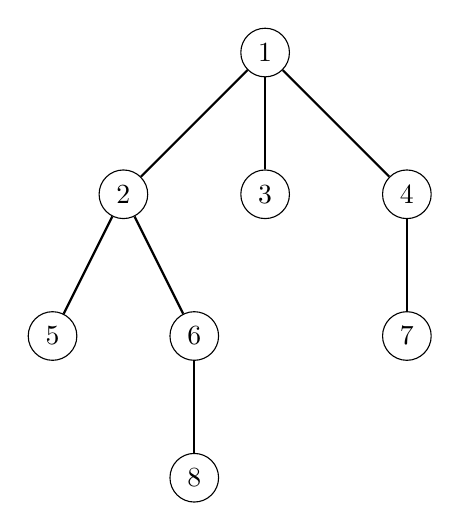
\begin{tikzpicture}[scale=0.9]
\node[draw, circle] (1) at (0,3) {$1$};
\node[draw, circle] (4) at (2,1) {$4$};
\node[draw, circle] (2) at (-2,1) {$2$};
\node[draw, circle] (3) at (0,1) {$3$};
\node[draw, circle] (7) at (2,-1) {$7$};
\node[draw, circle] (5) at (-3,-1) {$5$};
\node[draw, circle] (6) at (-1,-1) {$6$};
\node[draw, circle] (8) at (-1,-3) {$8$};
\path[draw,thick,-] (1) -- (2);
\path[draw,thick,-] (1) -- (3);
\path[draw,thick,-] (1) -- (4);
\path[draw,thick,-] (2) -- (5);
\path[draw,thick,-] (2) -- (6);
\path[draw,thick,-] (4) -- (7);
\path[draw,thick,-] (6) -- (8);
\end{tikzpicture}
\end{center}
\index{hijo}
\index{padre}

En un árbol enraizado, los \key{hijos} de un nodo
son sus vecinos inferiores, y el \key{padre} de un nodo
es su vecino superior.
Cada nodo tiene exactamente un padre,
excepto por la raíz que no tiene padre.
Por ejemplo, en el árbol anterior,
los hijos del nodo 2 son los nodos 5 y 6,
y su padre es el nodo 1.

\index{subárbol}

La estructura de un árbol enraizado es \emph{recursiva}:
cada nodo del árbol actúa como la raíz de un \key{subárbol}
que contiene el nodo mismo y todos los nodos
que están en los subárboles de sus hijos.
Por ejemplo, en el árbol anterior, el subárbol del nodo 2
contiene los nodos 2, 5, 6 y 8:
\begin{center}
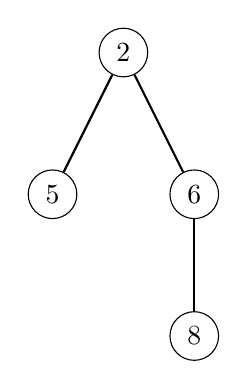
\begin{tikzpicture}[scale=0.9]
\node[draw, circle] (2) at (-2,1) {$2$};
\node[draw, circle] (5) at (-3,-1) {$5$};
\node[draw, circle] (6) at (-1,-1) {$6$};
\node[draw, circle] (8) at (-1,-3) {$8$};
\path[draw,thick,-] (2) -- (5);
\path[draw,thick,-] (2) -- (6);
\path[draw,thick,-] (6) -- (8);
\end{tikzpicture}
\end{center}

\section{Recorrido de árbol}

Los algoritmos de recorrido de grafo general
se pueden utilizar para recorrer los nodos de un árbol.
Sin embargo, el recorrido de un árbol es más fácil de implementar que
el de un grafo general, porque
no hay ciclos en el árbol y no es
posible alcanzar un nodo desde múltiples direcciones.

La forma típica de recorrer un árbol es comenzar
una búsqueda en profundidad en un nodo arbitrario.
La siguiente función recursiva se puede usar:

\begin{lstlisting}
void dfs(int s, int e) {
    // procesar nodo s
    for (auto u : adj[s]) {
        if (u != e) dfs(u, s);
    }
}
\end{lstlisting}

La función recibe dos parámetros: el nodo actual $s$
y el nodo anterior $e$.
El propósito del parámetro $e$ es asegurar
que la búsqueda solo se mueva a nodos
que no se han visitado todavía.

La siguiente llamada de función inicia la búsqueda
en el nodo $x$:

\begin{lstlisting}
dfs(x, 0);
\end{lstlisting}

En la primera llamada $e=0$, porque no hay
nodo anterior, y se permite
proceder a cualquier dirección en el árbol.

\subsubsection{Programación dinámica}

La programación dinámica se puede utilizar para calcular
alguna información durante un recorrido de árbol.
Usando programación dinámica, podemos, por ejemplo,
calcular en tiempo $O(n)$ para cada nodo de un árbol enraizado
la cantidad de nodos en su subárbol
o la longitud del camino más largo desde el nodo
a una hoja.

Como ejemplo, calculemos para cada nodo $s$
un valor $\texttt{count}[s]$: la cantidad de nodos en su subárbol.
El subárbol contiene el nodo mismo y
todos los nodos en los subárboles de sus hijos,
por lo que podemos calcular la cantidad de nodos
recursivamente usando el siguiente código:

\begin{lstlisting}
void dfs(int s, int e) {
    count[s] = 1;
    for (auto u : adj[s]) {
        if (u == e) continue;
        dfs(u, s);
        count[s] += count[u];
    }
}
\end{lstlisting}

\section{Diámetro}

\index{diámetro}
El \key{diámetro} de un árbol
es la longitud máxima de un camino entre dos nodos.
Por ejemplo, considera el siguiente árbol:
\begin{center}
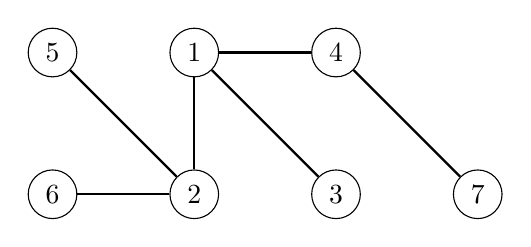
\begin{tikzpicture}[scale=0.9]
\node[draw, circle] (1) at (0,3) {$1$};
\node[draw, circle] (2) at (2,3) {$4$};
\node[draw, circle] (3) at (0,1) {$2$};
\node[draw, circle] (4) at (2,1) {$3$};
\node[draw, circle] (5) at (4,1) {$7$};
\node[draw, circle] (6) at (-2,3) {$5$};
\node[draw, circle] (7) at (-2,1) {$6$};
\path[draw,thick,-] (1) -- (2);
\path[draw,thick,-] (1) -- (3);
\path[draw,thick,-] (1) -- (4);
\path[draw,thick,-] (2) -- (5);
\path[draw,thick,-] (3) -- (6);
\path[draw,thick,-] (3) -- (7);
\end{tikzpicture}
\end{center}
El diámetro de este árbol es 4,
lo que corresponde al siguiente camino:
\begin{center}
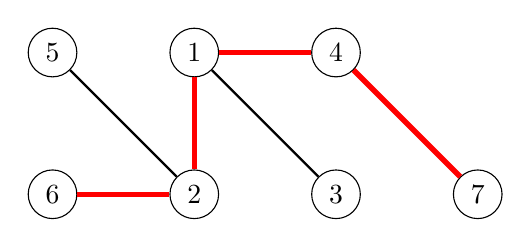
\begin{tikzpicture}[scale=0.9]
\node[draw, circle] (1) at (0,3) {$1$};
\node[draw, circle] (2) at (2,3) {$4$};
\node[draw, circle] (3) at (0,1) {$2$};
\node[draw, circle] (4) at (2,1) {$3$};
\node[draw, circle] (5) at (4,1) {$7$};
\node[draw, circle] (6) at (-2,3) {$5$};
\node[draw, circle] (7) at (-2,1) {$6$};
\path[draw,thick,-] (1) -- (2);
\path[draw,thick,-] (1) -- (3);
\path[draw,thick,-] (1) -- (4);
\path[draw,thick,-] (2) -- (5);
\path[draw,thick,-] (3) -- (6);
\path[draw,thick,-] (3) -- (7);

\path[draw,thick,-,color=red,line width=2pt] (7) -- (3);
\path[draw,thick,-,color=red,line width=2pt] (3) -- (1);
\path[draw,thick,-,color=red,line width=2pt] (1) -- (2);
\path[draw,thick,-,color=red,line width=2pt] (2) -- (5);
\end{tikzpicture}
\end{center}
Tenga en cuenta que puede haber varios caminos de longitud máxima.
En el camino anterior, podríamos reemplazar el nodo 6 con el nodo 5
para obtener otro camino con longitud 4.

A continuación, discutiremos dos algoritmos de tiempo $O(n)$
para calcular el diámetro de un árbol.
El primer algoritmo se basa en la programación dinámica,
y el segundo algoritmo utiliza dos búsquedas en profundidad.

\subsubsection{Algoritmo 1}

Una forma general de abordar muchos problemas de árboles
es primero enraizar el árbol arbitrariamente.
Después de esto, podemos intentar resolver el problema
por separado para cada subárbol.
Nuestro primer algoritmo para calcular el diámetro
se basa en esta idea.

Una observación importante es que cada camino
en un árbol enraizado tiene un \emph{punto más alto}:
el nodo más alto que pertenece al camino.
Por lo tanto, podemos calcular para cada nodo la longitud
del camino más largo cuyo punto más alto es el nodo.
Uno de esos caminos corresponde al diámetro del árbol.

Por ejemplo, en el siguiente árbol,
el nodo 1 es el punto más alto en el camino
que corresponde al diámetro:
\begin{center}
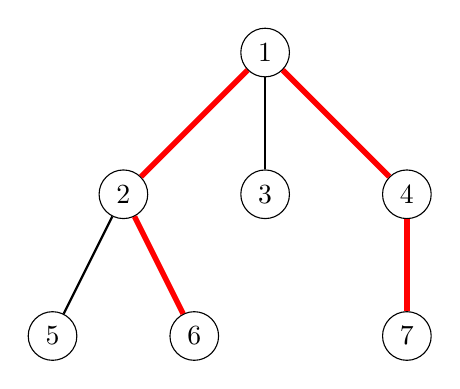
\begin{tikzpicture}[scale=0.9]
\node[draw, circle] (1) at (0,3) {$1$};
\node[draw, circle] (2) at (2,1) {$4$};
\node[draw, circle] (3) at (-2,1) {$2$};
\node[draw, circle] (4) at (0,1) {$3$};
\node[draw, circle] (5) at (2,-1) {$7$};
\node[draw, circle] (6) at (-3,-1) {$5$};
\node[draw, circle] (7) at (-1,-1) {$6$};
\path[draw,thick,-] (1) -- (2);
\path[draw,thick,-] (1) -- (3);
\path[draw,thick,-] (1) -- (4);
\path[draw,thick,-] (2) -- (5);
\path[draw,thick,-] (3) -- (6);
\path[draw,thick,-] (3) -- (7);

\path[draw,thick,-,color=red,line width=2pt] (7) -- (3);
\path[draw,thick,-,color=red,line width=2pt] (3) -- (1);
\path[draw,thick,-,color=red,line width=2pt] (1) -- (2);
\path[draw,thick,-,color=red,line width=2pt] (2) -- (5);
\end{tikzpicture}
\end{center}

Calculamos para cada nodo $x$ dos valores:
\begin{itemize}
\item $\texttt{toLeaf}(x)$: la longitud máxima de un camino desde $x$ hasta cualquier hoja
\item $\texttt{maxLength}(x)$: la longitud máxima de un camino
cuyo punto más alto es $x$
\end{itemize}
Por ejemplo, en el árbol anterior,
$\texttt{toLeaf}(1)=2$, porque hay un camino
$1 \rightarrow 2 \rightarrow 6$,
y $\texttt{maxLength}(1)=4$,
porque hay un camino
$6 \rightarrow 2 \rightarrow 1 \rightarrow 4 \rightarrow 7$.
En este caso, $\texttt{maxLength}(1)$ es igual al diámetro.

La programación dinámica se puede utilizar para calcular lo anterior
valores para todos los nodos en $O(n)$ tiempo.
Primero, para calcular $\texttt{toLeaf}(x)$,
recorremos los hijos de $x$,
elegimos un hijo $c$ con máximo $\texttt{toLeaf}(c)$
y sumamos uno a este valor.
Luego, para calcular $\texttt{maxLength}(x)$,
elegimos dos hijos distintos $a$ y $b$
de modo que la suma $\texttt{toLeaf}(a)+\texttt{toLeaf}(b)$
es máxima y sumamos dos a esta suma.

\subsubsection{Algoritmo 2}

Otra forma eficiente de calcular el diámetro
de un árbol se basa en dos búsquedas en profundidad.
Primero, elegimos un nodo arbitrario $a$ en el árbol
y encontramos el nodo más lejano $b$ de $a$.
Luego, encontramos el nodo más lejano $c$ de $b$.
El diámetro del árbol es la distancia entre $b$ y $c$.
En la siguiente gráfica, $a$, $b$ y $c$ podrían ser:
\begin{center}
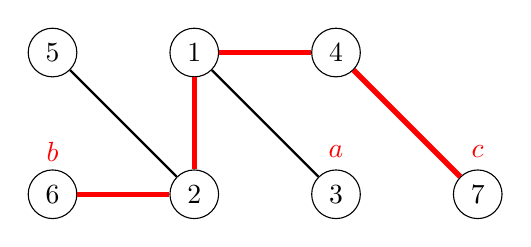
\begin{tikzpicture}[scale=0.9]
\node[draw, circle] (1) at (0,3) {$1$};
\node[draw, circle] (2) at (2,3) {$4$};
\node[draw, circle] (3) at (0,1) {$2$};
\node[draw, circle] (4) at (2,1) {$3$};
\node[draw, circle] (5) at (4,1) {$7$};
\node[draw, circle] (6) at (-2,3) {$5$};
\node[draw, circle] (7) at (-2,1) {$6$};
\path[draw,thick,-] (1) -- (2);
\path[draw,thick,-] (1) -- (3);
\path[draw,thick,-] (1) -- (4);
\path[draw,thick,-] (2) -- (5);
\path[draw,thick,-] (3) -- (6);
\path[draw,thick,-] (3) -- (7);
\node[color=red] at (2,1.6) {$a$};
\node[color=red] at (-2,1.6) {$b$};
\node[color=red] at (4,1.6) {$c$};

\path[draw,thick,-,color=red,line width=2pt] (7) -- (3);
\path[draw,thick,-,color=red,line width=2pt] (3) -- (1);
\path[draw,thick,-,color=red,line width=2pt] (1) -- (2);
\path[draw,thick,-,color=red,line width=2pt] (2) -- (5);
\end{tikzpicture}
\end{center}

Este es un método elegante, pero ¿por qué funciona?

Es útil dibujar el árbol de manera diferente para que
el camino que corresponde al diámetro
sea horizontal, y todos los demás
nodos cuelguen de él:
\begin{center}
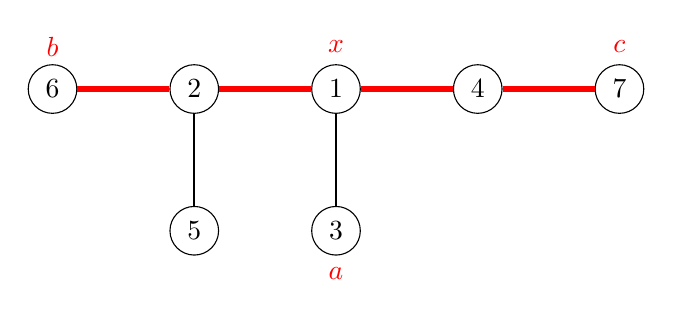
\begin{tikzpicture}[scale=0.9]
\node[draw, circle] (1) at (2,1) {$1$};
\node[draw, circle] (2) at (4,1) {$4$};
\node[draw, circle] (3) at (0,1) {$2$};
\node[draw, circle] (4) at (2,-1) {$3$};
\node[draw, circle] (5) at (6,1) {$7$};
\node[draw, circle] (6) at (0,-1) {$5$};
\node[draw, circle] (7) at (-2,1) {$6$};
\path[draw,thick,-] (1) -- (2);
\path[draw,thick,-] (1) -- (3);
\path[draw,thick,-] (1) -- (4);
\path[draw,thick,-] (2) -- (5);
\path[draw,thick,-] (3) -- (6);
\path[draw,thick,-] (3) -- (7);
\node[color=red] at (2,-1.6) {$a$};
\node[color=red] at (-2,1.6) {$b$};
\node[color=red] at (6,1.6) {$c$};
\node[color=red] at (2,1.6) {$x$};

\path[draw,thick,-,color=red,line width=2pt] (7) -- (3);
\path[draw,thick,-,color=red,line width=2pt] (3) -- (1);
\path[draw,thick,-,color=red,line width=2pt] (1) -- (2);
\path[draw,thick,-,color=red,line width=2pt] (2) -- (5);
\end{tikzpicture}
\end{center}

El nodo $x$ indica el lugar donde el camino
desde el nodo $a$ se une al camino que corresponde
al diámetro.
El nodo más lejano de $a$
es el nodo $b$, el nodo $c$ o algún otro nodo
que está al menos tan lejos del nodo $x$.
Por lo tanto, este nodo siempre es una opción válida para
un punto final de un camino que corresponde al diámetro.

\section{Todos los caminos más largos}

Nuestro próximo problema es calcular para cada nodo
en el árbol la longitud máxima de un camino
que comienza en el nodo.
Esto se puede ver como una generalización de la
problema de diámetro del árbol, porque el mayor de esos
longitudes es igual al diámetro del árbol.
También este problema se puede resolver en $O(n)$ tiempo.

Como ejemplo, considere el siguiente árbol:
\begin{center}
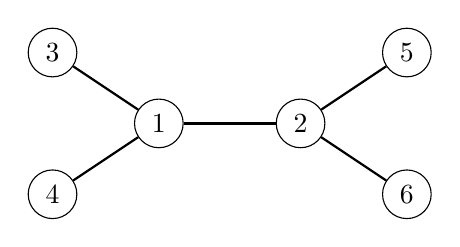
\begin{tikzpicture}[scale=0.9]
\node[draw, circle] (1) at (0,0) {$1$};
\node[draw, circle] (2) at (-1.5,-1) {$4$};
\node[draw, circle] (3) at (2,0) {$2$};
\node[draw, circle] (4) at (-1.5,1) {$3$};
\node[draw, circle] (6) at (3.5,-1) {$6$};
\node[draw, circle] (7) at (3.5,1) {$5$};
\path[draw,thick,-] (1) -- (2);
\path[draw,thick,-] (1) -- (3);
\path[draw,thick,-] (1) -- (4);
\path[draw,thick,-] (3) -- (6);
\path[draw,thick,-] (3) -- (7);
\end{tikzpicture}
\end{center}

Sea $\texttt{maxLength}(x)$ denotar la longitud máxima
de un camino que comienza en el nodo $x$.
Por ejemplo, en el árbol de arriba,
$\texttt{maxLength}(4)=3$, porque hay
un camino $4 \rightarrow 1 \rightarrow 2 \rightarrow 6$.
Aquí hay una tabla completa de los valores:
\begin{center}
\begin{tabular}{l|lllllll}
nodo $x$ & 1 & 2 & 3 & 4 & 5 & 6 \\
$\texttt{maxLength}(x)$ & 2 & 2 & 3 & 3 & 3 & 3 \\
\end{tabular}
\end{center}

También en este problema, un buen punto de partida
para resolver el problema es enraizar el árbol arbitrariamente:
\begin{center}
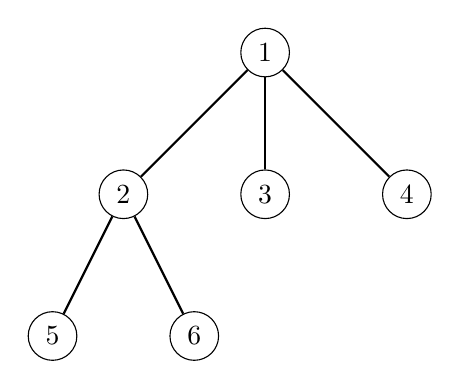
\begin{tikzpicture}[scale=0.9]
\node[draw, circle] (1) at (0,3) {$1$};
\node[draw, circle] (2) at (2,1) {$4$};
\node[draw, circle] (3) at (-2,1) {$2$};
\node[draw, circle] (4) at (0,1) {$3$};
\node[draw, circle] (6) at (-3,-1) {$5$};
\node[draw, circle] (7) at (-1,-1) {$6$};
\path[draw,thick,-] (1) -- (2);
\path[draw,thick,-] (1) -- (3);
\path[draw,thick,-] (1) -- (4);
\path[draw,thick,-] (3) -- (6);
\path[draw,thick,-] (3) -- (7);
\end{tikzpicture}
\end{center}

La primera parte del problema es calcular para cada nodo $x$
la longitud máxima de un camino que pasa por un hijo de $x$.
Por ejemplo, el camino más largo desde el nodo 1
pasa por su hijo 2:
\begin{center}
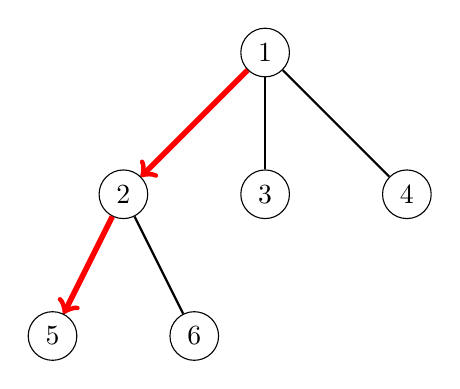
\begin{tikzpicture}[scale=0.9]
\node[draw, circle] (1) at (0,3) {$1$};
\node[draw, circle] (2) at (2,1) {$4$};
\node[draw, circle] (3) at (-2,1) {$2$};
\node[draw, circle] (4) at (0,1) {$3$};
\node[draw, circle] (6) at (-3,-1) {$5$};
\node[draw, circle] (7) at (-1,-1) {$6$};
\path[draw,thick,-] (1) -- (2);
\path[draw,thick,-] (1) -- (3);
\path[draw,thick,-] (1) -- (4);
\path[draw,thick,-] (3) -- (6);
\path[draw,thick,-] (3) -- (7);

\path[draw,thick,->,color=red,line width=2pt] (1) -- (3);
\path[draw,thick,->,color=red,line width=2pt] (3) -- (6);
\end{tikzpicture}
\end{center}
Esta parte es fácil de resolver en tiempo $O(n)$, porque podemos usar
programación dinámica como lo hemos hecho anteriormente.

Luego, la segunda parte del problema es calcular
para cada nodo $x$ la longitud máxima de una ruta
a través de su padre $p$.
Por ejemplo, la ruta más larga
desde el nodo 3 pasa por su padre 1:
\begin{center}
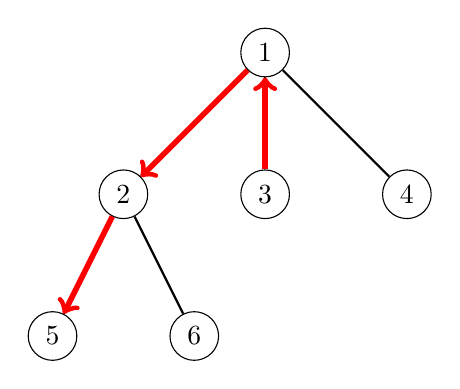
\begin{tikzpicture}[scale=0.9]
\node[draw, circle] (1) at (0,3) {$1$};
\node[draw, circle] (2) at (2,1) {$4$};
\node[draw, circle] (3) at (-2,1) {$2$};
\node[draw, circle] (4) at (0,1) {$3$};
\node[draw, circle] (6) at (-3,-1) {$5$};
\node[draw, circle] (7) at (-1,-1) {$6$};
\path[draw,thick,-] (1) -- (2);
\path[draw,thick,-] (1) -- (3);
\path[draw,thick,-] (1) -- (4);
\path[draw,thick,-] (3) -- (6);
\path[draw,thick,-] (3) -- (7);

\path[draw,thick,->,color=red,line width=2pt] (4) -- (1);
\path[draw,thick,->,color=red,line width=2pt] (1) -- (3);
\path[draw,thick,->,color=red,line width=2pt] (3) -- (6);
\end{tikzpicture}
\end{center}

A primera vista, parece que deberíamos elegir
la ruta más larga desde $p$.
Sin embargo, esto \emph{no} siempre funciona,
porque la ruta más larga desde $p$
puede pasar por $x$.
Aquí hay un ejemplo de esta situación:
\begin{center}
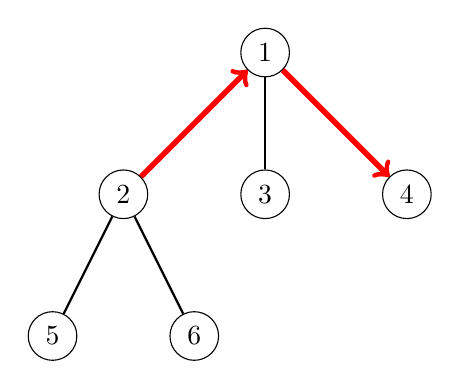
\begin{tikzpicture}[scale=0.9]
\node[draw, circle] (1) at (0,3) {$1$};
\node[draw, circle] (2) at (2,1) {$4$};
\node[draw, circle] (3) at (-2,1) {$2$};
\node[draw, circle] (4) at (0,1) {$3$};
\node[draw, circle] (6) at (-3,-1) {$5$};
\node[draw, circle] (7) at (-1,-1) {$6$};
\path[draw,thick,-] (1) -- (2);
\path[draw,thick,-] (1) -- (3);
\path[draw,thick,-] (1) -- (4);
\path[draw,thick,-] (3) -- (6);
\path[draw,thick,-] (3) -- (7);

\path[draw,thick,->,color=red,line width=2pt] (3) -- (1);
\path[draw,thick,->,color=red,line width=2pt] (1) -- (2);
\end{tikzpicture}
\end{center}

Aún así, podemos resolver la segunda parte en
tiempo $O(n)$ almacenando \emph{dos} longitudes máximas
para cada nodo $x$:
\begin{itemize}
\item $\texttt{maxLength}_1(x)$:
la longitud máxima de una ruta desde $x$
\item $\texttt{maxLength}_2(x)$
la longitud máxima de una ruta desde $x$
en otra dirección que la primera ruta
\end{itemize}
Por ejemplo, en el gráfico anterior,
$\texttt{maxLength}_1(1)=2$
usando la ruta $1 \rightarrow 2 \rightarrow 5$,
y $\texttt{maxLength}_2(1)=1$
usando la ruta $1 \rightarrow 3$.

Finalmente, si la ruta que corresponde a
$\texttt{maxLength}_1(p)$ pasa por $x$,
concluimos que la longitud máxima es
$\texttt{maxLength}_2(p)+1$,
y de lo contrario la longitud máxima es
$\texttt{maxLength}_1(p)+1$.


\section{Árboles binarios}

\index{árbol binario}

\begin{samepage}
Un \key{árbol binario} es un árbol enraizado
donde cada nodo tiene un subárbol izquierdo y derecho.
Es posible que un subárbol de un nodo esté vacío.
Por lo tanto, cada nodo en un árbol binario tiene
cero, uno o dos hijos.

Por ejemplo, el siguiente árbol es un árbol binario:
\begin{center}
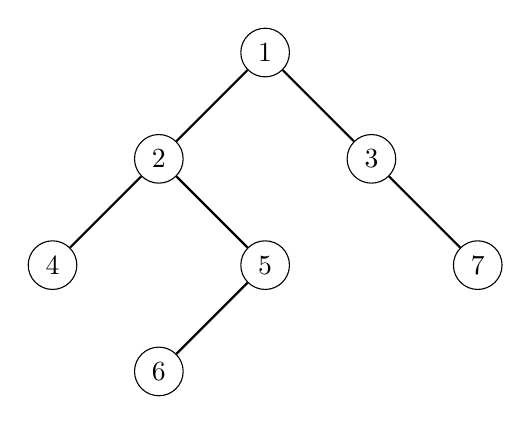
\begin{tikzpicture}[scale=0.9]
\node[draw, circle] (1) at (0,0) {$1$};
\node[draw, circle] (2) at (-1.5,-1.5) {$2$};
\node[draw, circle] (3) at (1.5,-1.5) {$3$};
\node[draw, circle] (4) at (-3,-3) {$4$};
\node[draw, circle] (5) at (0,-3) {$5$};
\node[draw, circle] (6) at (-1.5,-4.5) {$6$};
\node[draw, circle] (7) at (3,-3) {$7$};

\path[draw,thick,-] (1) -- (2);
\path[draw,thick,-] (1) -- (3);
\path[draw,thick,-] (2) -- (4);
\path[draw,thick,-] (2) -- (5);
\path[draw,thick,-] (5) -- (6);
\path[draw,thick,-] (3) -- (7);
\end{tikzpicture}
\end{center}
\end{samepage}

\index{preorden}
\index{en orden}
\index{posorden}

Los nodos de un árbol binario tienen tres ordenamientos naturales
que corresponden a diferentes formas de
recorrer el árbol recursivamente:

\begin{itemize}
\item \key{preorden}: primero procesa la raíz,
luego recorre el subárbol izquierdo, luego recorre el subárbol derecho
\item \key{en orden}: primero recorre el subárbol izquierdo,
luego procesa la raíz, luego recorre el subárbol derecho
\item \key{posorden}: primero recorre el subárbol izquierdo,
luego recorre el subárbol derecho, luego procesa la raíz
\end{itemize}

Para el árbol anterior, los nodos en
preorden son
$[1,2,4,5,6,3,7]$,
en en orden $[4,2,6,5,1,3,7]$
y en posorden $[4,6,5,2,7,3,1]$.

Si sabemos el preorden y el en orden
de un árbol, podemos reconstruir la estructura exacta del árbol.
Por ejemplo, el árbol anterior es el único árbol posible
con preorden $[1,2,4,5,6,3,7]$ y
en orden $[4,2,6,5,1,3,7]$.
De manera similar, el posorden y el en orden
también determinan la estructura de un árbol.

Sin embargo, la situación es diferente si solo conocemos
el preorden y el posorden de un árbol.
En este caso, puede haber más de un árbol
que coincida con los ordenamientos.
Por ejemplo, en ambos árboles
\begin{center}
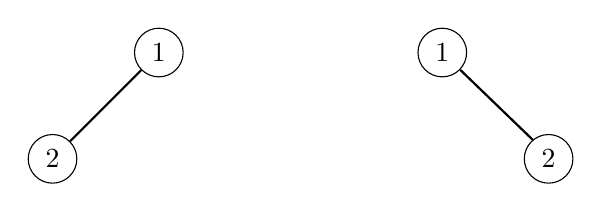
\begin{tikzpicture}[scale=0.9]
\node[draw, circle] (1) at (0,0) {$1$};
\node[draw, circle] (2) at (-1.5,-1.5) {$2$};
\path[draw,thick,-] (1) -- (2);

\node[draw, circle] (1b) at (0+4,0) {$1$};
\node[draw, circle] (2b) at (1.5+4,-1.5) {$2$};
\path[draw,thick,-] (1b) -- (2b);
\end{tikzpicture}
\end{center}
el preorden es $[1,2]$ y el postorden es $[2,1]$,
pero las estructuras de los árboles son diferentes. 
